% ------------------------------------------------------------------------
% ------------------------------------------------------------------------
% abnTeX2: Modelo de Trabalho Academico (tese de doutorado, dissertacao de
% mestrado e trabalhos monograficos em geral) em conformidade com
% ABNT NBR 14724:2011: Informacao e documentacao - Trabalhos academicos -
% Apresentacao
% ------------------------------------------------------------------------
% ------------------------------------------------------------------------

\documentclass[
% -- opções da classe memoir --
12pt, % tamanho da fonte
openright, % capítulos começam em pág ímpar (insere página vazia caso preciso)
oneside, % para impressão em verso e anverso. Oposto a twoside
a4paper, % tamanho do papel.
% -- opções da classe abntex2 --
%chapter=TITLE, % títulos de capítulos convertidos em letras maiúsculas
%section=TITLE, % títulos de seções convertidos em letras maiúsculas
%subsection=TITLE, % títulos de subseções convertidos em letras maiúsculas
%subsubsection=TITLE,% títulos de subsubseções convertidos em letras maiúsculas
% -- opções do pacote babel --
english, % idioma adicional para hifenização
brazil, % o último idioma é o principal do documento
]{abntex2}


% ---
% Pacotes fundamentais
% ---
\usepackage{cite}
\usepackage[brazil]{babel}
\usepackage{cmap}	% Mapear caracteres especiais no PDF
\usepackage{lmodern}	% Usa a fonte Latin Modern
\usepackage[T1]{fontenc}	% Selecao de codigos de fonte.
\usepackage[utf8]{inputenc}	% Codificacao do documento (conversão automática dos acentos)
\usepackage{lastpage}	% Usado pela Ficha catalográfica
\usepackage{indentfirst}	% Indenta o primeiro parágrafo de cada seção.
\usepackage{color}	% Controle das cores
\usepackage{graphicx}	% Inclusão de gráficos
\usepackage{float}
\usepackage{hyperref}
\usepackage{listings}

% ---
% Pacotes adicionais, usados apenas no âmbito do Modelo Canônico do abnteX2
% ---
\usepackage{lipsum}	% para geração de dummy text
% ---

% ---
% Pacotes de citações
% ---
\usepackage[brazilian,hyperpageref]{backref}	% Paginas com as citações na bibl
\usepackage[alf]{abntex2cite}	% Citações padrão ABNT

% ---
% CONFIGURAÇÕES DE PACOTES
% ---

% ---
% Configurações do pacote backref
% Usado sem a opção hyperpageref de backref
\renewcommand{\backrefpagesname}{Citado na(s) página(s):~}
% Texto padrão antes do número das páginas
\renewcommand{\backref}{}
% Define os textos da citação
\renewcommand*{\backrefalt}[4]{
\ifcase #1 %
Nenhuma citação no texto.%
\or
Citado na página #2.%
\else
Citado #1 vezes nas páginas #2.%
\fi}%
% ---


% ---
% Informações de dados para CAPA e FOLHA DE ROSTO
% ---
\titulo{Paradigmas de Programação da linguagem LUA}
\autor{Mário Sérgio Oliveira de Queiroz \\ Pedro Martins}
\local{Brasil}
\data{25 de Novembro de 2013}
\orientador{João Paulo Ataíde Martins}
\instituicao{%
  IESB - Centro Universitário Instituto de Ensino Superior de Brasília
  \par
  Ciência da Computação}
\tipotrabalho{TCC (Graduação)}
% O preambulo deve conter o tipo do trabalho, o objetivo,
% o nome da instituição e a área de concentração
\preambulo{Projeto para a disciplina Projeto Integrador VI - Paradigmas de Linguagem de Programação,
do Centro Universitário Instituto de Educação Superior de Brasília, DF.}
% ---


% ---
% Configurações de aparência do PDF final

% alterando o aspecto da cor azul
\definecolor{blue}{RGB}{41,5,195}

% informações do PDF
\makeatletter
\hypersetup{
      %pagebackref=true,
pdftitle={\@title},
pdfauthor={\@author},
     pdfsubject={\imprimirpreambulo},
pdfcreator={LaTeX with abnTeX2},
pdfkeywords={abnt}{latex}{abntex}{abntex2}{trabalho acadêmico},
colorlinks=true, % false: boxed links; true: colored links
     linkcolor=black, % color of internal links
     citecolor=black, % color of links to bibliography
     filecolor=magenta, % color of file links
urlcolor=blue,
bookmarksdepth=4
}
\makeatother
% ---

% ---
% Espaçamentos entre linhas e parágrafos
% ---

% O tamanho do parágrafo é dado por:
\setlength{\parindent}{1.3cm}

% Controle do espaçamento entre um parágrafo e outro:
\setlength{\parskip}{0.2cm} % tente também \onelineskip

% ---
% compila o indice
% ---
\makeindex
% ---

% ----
% Início do documento
% ----
\begin{document}

% Retira espaço extra obsoleto entre as frases.
\frenchspacing

% ----------------------------------------------------------
% ELEMENTOS PRÉ-TEXTUAIS
% ----------------------------------------------------------
% \pretextual

% ---
% Capa
% ---
\imprimircapa
% ---

% ---
% Folha de rosto
% (o * indica que haverá a ficha bibliográfica)
% ---
\imprimirfolhaderosto*
% ---

% ---
% Inserir a ficha bibliografica
% ---

% Isto é um exemplo de Ficha Catalográfica, ou ``Dados internacionais de
% catalogação-na-publicação''. Você pode utilizar este modelo como referência.
% Porém, provavelmente a biblioteca da sua universidade lhe fornecerá um PDF
% com a ficha catalográfica definitiva após a defesa do trabalho. Quando estiver
% com o documento, salve-o como PDF no diretório do seu projeto e substitua todo
% o conteúdo de implementação deste arquivo pelo comando abaixo:
%
\begin{fichacatalografica}
\vspace*{\fill}	% Posição vertical
\hrule	% Linha horizontal
\begin{center}	% Minipage Centralizado
\begin{minipage}[c]{12.5cm}	% Largura

\imprimirautor

\hspace{0.5cm} \imprimirtitulo. --
\imprimirlocal, \imprimirdata-

\hspace{0.5cm} \pageref{LastPage} p.\\

\hspace{0.5cm} \imprimirorientadorRotulo~\imprimirorientador\\

\hspace{0.5cm}
\parbox[t]{\textwidth}{\imprimirtipotrabalho~--~\imprimirinstituicao,
\imprimirdata.}\\

\hspace{0.5cm}
1. Lua.
2. Paradigmas.
I. João Paulo.
II. IESB.
III. Ciência da Computação.

\hspace{8.75cm} CDU 02:141:005.7\\

\end{minipage}
\end{center}
\hrule
\end{fichacatalografica}
% ---

% ---
% Inserir folha de aprovação
% ---

% Isto é um exemplo de Folha de aprovação, elemento obrigatório da NBR
% 14724/2011 (seção 4.2.1.3). Você pode utilizar este modelo até a aprovação
% do trabalho. Após isso, substitua todo o conteúdo deste arquivo por uma
% imagem da página assinada pela banca com o comando abaixo:
%
\begin{folhadeaprovacao}

  \begin{center}
    {\ABNTEXchapterfont\large\imprimirautor}

    \vspace*{\fill}\vspace*{\fill}
    {\ABNTEXchapterfont\bfseries\Large\imprimirtitulo}
    \vspace*{\fill}
    
    \hspace{.45\textwidth}
    \begin{minipage}{.5\textwidth}
        \imprimirpreambulo
    \end{minipage}%
    \vspace*{\fill}
   \end{center}
    
   Trabalho aprovado. \imprimirlocal, \imprimirdata:

   \assinatura{\textbf{\imprimirorientador} \\ Orientador}
   \assinatura{\textbf{Professor} \\ Convidado 1}
   \assinatura{\textbf{Professor} \\ Convidado 2}
      
   \begin{center}
    \vspace*{0.5cm}
    {\large\imprimirlocal}
    \par
    {\large\imprimirdata}
    \vspace*{1cm}
  \end{center}
  
\end{folhadeaprovacao}
% ---

% ---
% Dedicatória
% ---
\begin{dedicatoria}
   \vspace*{\fill}
   \centering
   \noindent
   \textit{ Este trabalho é dedicado às crianças adultas que,\\
   quando pequenas, sonharam em se tornar cientistas.} \vspace*{\fill}
\end{dedicatoria}
% ---

% ---
% Agradecimentos
% ---
\begin{agradecimentos}
Os agradecimentos principais são direcionados à Gerald Weber, Miguel Frasson,
Leslie H. Watter, Bruno Parente Lima, Flávio de Vasconcellos Corrêa, Otavio Real
Salvador, Renato Machnievscz\footnote{Os nomes dos integrantes do primeiro
projeto abn\TeX\ foram extraídos de
\url{http://codigolivre.org.br/projects/abntex/}} e todos aqueles que
contribuíram para que a produção de trabalhos acadêmicos conforme
as normas ABNT com \LaTeX\ fosse possível.

Agradecimentos especiais são direcionados ao Centro de Pesquisa em Arquitetura
da Informação\footnote{\url{http://www.cpai.unb.br/}} da Universidade de
Brasília (CPAI), ao grupo de usuários
\emph{latex-br}\footnote{\url{http://groups.google.com/group/latex-br}} e aos
novos voluntários do grupo
\emph{\abnTeX}\footnote{\url{http://groups.google.com/group/abntex2} e
\url{http://abntex2.googlecode.com/}}~que contribuíram e que ainda
contribuirão para a evolução do \abnTeX.

\end{agradecimentos}

% ---
% Epígrafe
% ---
\begin{epigrafe}
    \vspace*{\fill}
\begin{flushright}
\textit{``Tudo tem o seu tempo determinado, \\
e há tempo para todo o propósito debaixo do céu. \\
Há tempo de nascer, e tempo de morrer; \\
tempo de plantar, e tempo de arrancar o que se plantou\\
(Bíblia Sagrada, Eclesiastes 3, 1 e 2)}
\end{flushright}
\end{epigrafe}
% % ---

% ---
% RESUMOS
% ---

% resumo em português
\begin{resumo}
 Este projeto se refere à estudos e pesquisas, relativas aos paradigmas e conceitos da linguagem de programação Lua. 

 Para isso, foi utilizado a documentação oficial da linguagem como base contida em \cite{Lua_Org}, e os conceitos relacionados a projetos de linguagem de programação do livro \cite{Sebesta}. Como ferramentas para a elaboração do trabalho foi utilizado o latex para a parte de documentação e o sublime para a execução de códigos Lua.

 Com base no que foi mencionado, o projeto deseja abordar todos os conceitos e paradigmas da linguagem de programação Lua.

 \noindent
 \textbf{Palavras-chaves}: latex. abntex. editoração de texto.
\end{resumo}

% resumo em inglês
\begin{resumo}[Abstract]
 \begin{otherlanguage*}{english}
   This is the english abstract.

   \vspace{\onelineskip}
 
   \noindent
   \textbf{Key-words}: latex. abntex. text editoration.
 \end{otherlanguage*}
\end{resumo}

% ---
% inserir lista de ilustrações
% ---
\pdfbookmark[0]{\listfigurename}{lof}
\listoffigures*
\cleardoublepage
% ---

% ---
% inserir lista de tabelas
% ---
\pdfbookmark[0]{\listtablename}{lot}
\listoftables*
\cleardoublepage
% ---

% ---
% inserir lista de abreviaturas e siglas
% ---
\begin{siglas}
  \item[TV] Televisão 
  \item[PUC-Rio] Pontifícia Universidade Católica do Rio de Janeiro
  \item[Tecgraf] Instituto de Desenvolvimento de Software Técnico-Científico PUC-Rio
  \item[LabLua] Laboratório de desenvolvimento da linguagem Lua
  \item[PETROBRAS]  Petróleo Brasileiro S.A. 
  \item[DEL] Linguagem para Especificação de Diálogos 
  \item[SOL] Simple Object Language
  \item[BSD] Berkeley Software Distribution 
  \item[MIT] Massachusetts Institute of Technology
  \item[BNF] Formalismo de Backus-Naur
\end{siglas}
% ---

% ---
% inserir lista de símbolos
% ---
% \begin{simbolos}
%   \item[$ \Gamma $] Letra grega Gama
%   \item[$ \Lambda $] Lambda
%   \item[$ \zeta $] Letra grega minúscula zeta
%   \item[$ \in $] Pertence
% \end{simbolos}
% ---

% ---
% inserir o sumario
% ---
\pdfbookmark[0]{\contentsname}{toc}
\tableofcontents*
\cleardoublepage
% ---

% ----------------------------------------------------------
% ELEMENTOS TEXTUAIS
% ----------------------------------------------------------
\textual

% ----------------------------------------------------------
% Introdução
% ----------------------------------------------------------
\chapter{Introdução}
Este trabalho acadêmico se refere ao desenvolvimento de um estudo e pesquisa, relativo aos paradigmas e conceitos da linguagem de programação Lua. Desta forma, serão atingidos temas como implementação de sintaxe e semântica da linguagem.

\section{Motivação}
Conforme a proposta de projeto para o semestre, no que se refere ao estudo dos paradigmas de uma linguagem de programação, a escolha do grupo pela linguagem Lua, teve vários estímulos, como o fato da linguagem ter surgido em uma universidade brasileira, além de possuir uma ampla aplicação no ambiente de jogos e na indústria de TV digital.

Em virtude do que foi mencionado, existiram muitas influências para a escolha de Lua para esse projeto, existia o interesse em outras linguagens como Python, más devido as outras escolhas, optamos por Lua, que inclusive temos algumas experiências de trabalho.

\section{Objetivos}

\subsection{Geral}
Este trabalho tem como objetivo aplicar os conhecimentos obtidos na disciplina de paradigmas de linguagem de programação à linguagem Lua. Aprofundar e colocar em prática os conceitos aprendidos em sala de aula, documentando e exemplificando o funcionamento da linguagem Lua.

\subsection{Específicos}
Com base no objetivo geral derivam-se os seguintes objetivos específicos.
\begin{itemize}
\item Embasar historicamente a linguagem.
\item Explicar o funcionamento da sintaxe e semântica.
\item Demonstrar os paradigmas envolvidos na linguagem.
\item Explicar e exemplificar o funcionamento de variáveis. Incluindo os tipos, sua vinculação, verificação de tipo e escopo.
\item Apresentar as vantagens, desvantagens e as áreas a qual Lua melhor se aplica.
\item Criar códigos para exemplificar os conceitos apresentados.
\end{itemize}

% \section{Organização do Trabalho}


% ----------------------------------------------------------
% Capitulo com exemplos de comandos inseridos de arquivo externo
% ----------------------------------------------------------

\include{abntex2-modelo-include-comandos}

% ---
% Capitulo de revisão de literatura
% ---
\chapter{Histórico}
A linguagem Lua foi totalmente projetada, e implementada no Brasil, por Roberto Ierusalimschy, Luiz Henrique de Figueiredo e Waldemar Celes, que eram membros do Computer Graphics Technology Group na PUC-Rio, a Pontifícia Universidade Católica do Rio de Janeiro. Lua nasceu e cresceu no Tecgraf, Grupo de Tecnologia em Computação Gráfica da PUC-Rio. Atualmente, Lua é desenvolvida no laboratório LabLua. Tanto o Tecgraf quanto Lablua são laboratórios do Departamento de Informática da PUC-Rio.

O estímulo inicial para a construção da linguagem veio de um projeto entre a PETROBRAS e a PUC-RIO, a fim de produzir um programa de interfaces gráficas para várias aplicações.

\begin{figure}[H]
\centering
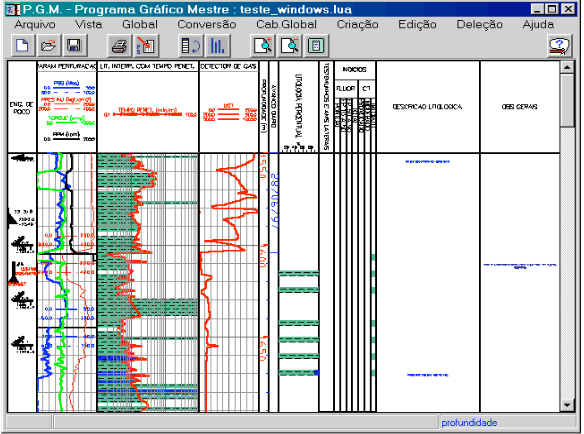
\includegraphics[width=0.5\linewidth]{imagens/imagem1.png}
\caption{Programa Gráfico Mestre}
\end{figure}

Logo surgiu o primeiro protótipo, DEL - Linguagem para Especificação de Diálogos, que trabalhava com lista de parâmetros e tipos e valores padrões. Com o passar do tempo após pesquisas e mudanças no projeto surgiu a linguagem `SOL' - Simple Object Language, sendo que era uma linguagem para descrição de objetos, inspirada no bibTex.

\begin{figure}[H]
\centering
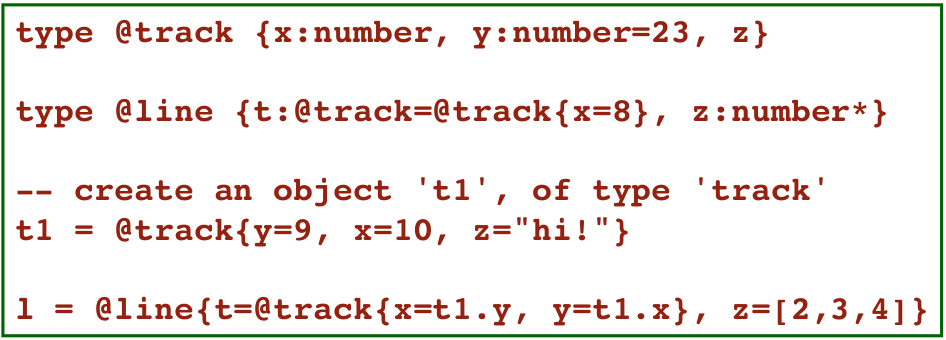
\includegraphics[width=0.5\linewidth]{imagens/imagem2.png}
\caption{Trecho de código da linguagem SOL}
\end{figure}

No entanto, tanto DEL como SOL tinha várias limitações como, pouco recurso para construção de diálogos, pouca abstração de dados e incompleta se comparadas às linguagens contemporâneas a elas. Então Roberto Ierusalimschy, Luiz Henrique de Figueiredo e Waldemar Celes se juntaram para achar uma solução comum a seus problemas. As propostas de solução era formular uma nova linguagem de configuração genérica, que fosse facilmente acoplável, portável, simples e uma sintaxe fácil. Para o resultado desse projeto foi dado o nome LUA, como um contráste da antiga SOL.

As linguagens que mais se aproximam das características de Lua são o Icon, por sua concepção, e Python, por sua facilidade de utilização. Em um artigo publicado no Dr. Dobb's Journal, os criadores de Lua também afirmam que Lisp e Scheme foram de grande influência na decisão de desenvolver a tabela como a principal estrutura de dados de Lua. Lua tem sido usada em várias aplicações, tanto comerciais como não-comerciais.

Versões de Lua antes da versão 5.0 foram liberadas sob uma licença similar à licença BSD. A partir da versão 5.0, Lua foi licenciada sob a licença MIT.

Hoje a linguagem é uma das mais utilizadas do mundo estando entre as vinte mais utilizadas.

\chapter{Aspectos léxicos e sintáticos de Lua}
Esta capítulo descreve os principais aspectos léxicos, sintáticos e semânticos da linguagem Lua. sendo assim, serão descritas quais itens léxicos são válidos, como eles são combinados, e qual o significado da sua combinação.

O estudo de linguagens de programação pode ser orientado à verificação dos aspectos semânticos e sintáticos de uma linguagem. Pois a sintaxe é a forma das expressões e instruções, ou seja, como é feita a construção das mesmas. Não obstante, a semântica é o sforam ignificado das expressões e instruções.

\section{Convenções Léxicas}
Em Lua, os nomes podem ser qualquer cadeia de letras, dígitos, e sublinhados que não começam com um dígito, assim como em outras linguagens tradicionais, como C/C++. Os identificadores são usados para nomear variáveis e campos de tabelas.

Lua é uma linguagem que diferencia letras minúsculas de maiúsculas, por exemplo, and é uma palavra reservada, mas And e AND são dois nomes válidos diferentes. Como convenção, nomes que começam com um sublinhado seguido por letras maiúsculas são reservados para variáveis globais internas usadas por Lua.

As seguintes cadeias denotam outros itens léxicos:
+ - * == ~= <= >= < > = ( ) { } [ ] ; : , . .. ...

As cadeias de caracteres literais podem ser delimitadas através do uso de aspas simples ou aspas duplas, e podem conter as seguintes seqüências de escape no estilo de C: `contra-barra + a' (campainha), `contra-barra + b' (backspace), `contra-barra + f' (alimentação de formulário), `contra-barra + n' (quebra de linha), `contra-barra + r' (retorno de carro), `contra-barra + t' (tabulação horizontal), `contra-barra + v' (tabulação vertical), `contra-barra + contra-barra' (barra invertida), `contra-barra + aspas duplas' (citação [aspa dupla]) e `contra-barra + aspas simples'. Além disso, uma barra invertida seguida por uma quebra de linha real resulta em uma quebra de linha na cadeia de caracteres. Um caractere em uma cadeia de caracteres também pode ser especificado pelo seu valor numérico usando a seqüência de escape contra-barra + ddd, onde ddd é uma seqüência de até três dígitos decimais. (Note que se um caractere numérico representado como um seqüência de escape for seguido por um dígito, a seqüência de escape deve possuir exatamente três dígitos.) Cadeias de caracteres em Lua podem conter qualquer valor de 8 bits, incluindo zeros dentro delas, os quais podem ser especificados como `contra-barra + 0'.

Cadeias literais longas podem ser definidas usando um formato longo delimitado por colchetes. Definimos uma abertura de colchete longo de nível n como um abre colchete seguido por n sinais de igual seguido por outro abre colchete. Dessa forma, uma abertura de colchete longo de nível 0 é escrita como [[, uma abertura de colchete longo de nível 1 é escrita como [=[ e assim por diante. Um fechamento de colchete longo é definido de maneira similar. Uma cadeia de caracteres longa começa com uma abertura de colchete longo de qualquer nível e termina no primeiro fechamento de colchete longo do mesmo nível. Literais expressos desta forma podem se estender por várias linhas, não interpretam nenhuma seqüência de escape e ignoram colchetes longos de qualquer outro nível. Estes literais podem conter qualquer coisa, exceto um fechamento de colchete longo de nível igual ao da abertura.

As seguintes palavras-chave são reservadas e não podem ser utilizadas como nomes:
\begin{itemize}
\item and
\item break
\item do
\item else 
\item elseif
\item end
\item false
\item for
\item function
\item if
\item in
\item local
\item nil
\item not
\item or
\item repeat
\item return
\item then
\item true
\item until
\item while
\end{itemize}

\section{Sintaxe de Lua}
Aqui está a sintaxe completa de Lua na notação BNF estendida. (Ela não descreve as precedências dos operadores.)

\begin{figure}[H]
\centering
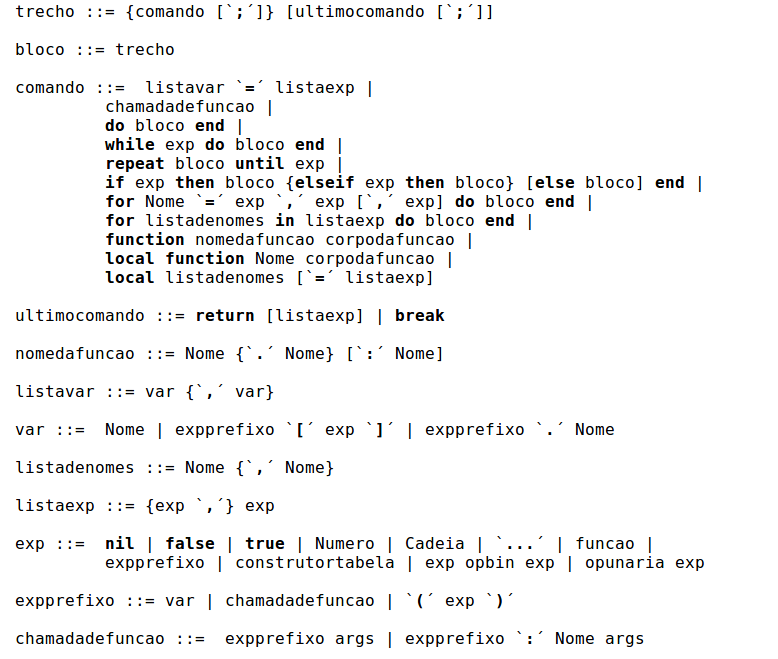
\includegraphics[width=0.9\linewidth]{imagens/sintaxe1.png}
\end{figure}

\begin{figure}[H]
\centering
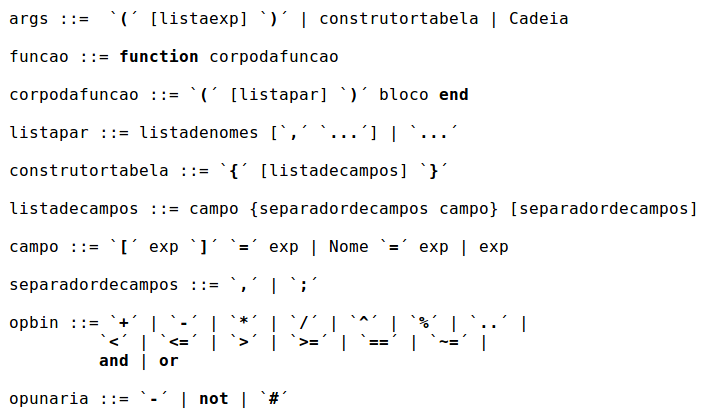
\includegraphics[width=0.9\linewidth]{imagens/sintaxe2.png}
\end{figure}


% ---
% segundo capitulo de Resultados
% ---
\chapter{Semântica das Variáveis}
Este capítulo apresenta as questões fundamentais das variáveis. Como tipo, endereço e valores. Além da abordagem de vinculação e de escopo.

\section{Variáveis}
Uma variável em uma linguagem é a abstração do conteúdo de células de memória do computador. Variáveis podem se caracterizadas de acordo com os seguintes aspectos: nome, endereço, valor, tipo, tempo de vida e escopo.

Em Lua existem três tipos de variáveis, sendo elas as seguites: variáveis globais, variáveis locais e variáveis de tabelas. Sendo que, a diferença entre variáveis locais e globais é o uso da palavra reservada `local' antes do nome da variável. Já as variáveis de tabela são os nomes dados aos índices das tabelas, tendo em vista que toda a estrutura de dados linguagem é orientada à tabelas.

\section{Vinculação}
O termo vinculação é uma associação ou uma referência, como, por exemplo, entre uma atributo e uma entidade e entre uma operação e um símbolo. O momento em que ocorre a vinculação é denominado como tempo de vinculação. Isso porquê, as vinculações podem ocorrer no tempo de projeto da linguagem, no tempo de implementação, no tempo de compilação, no tempo de ligação, no tempo de carregamento ou no tempo de execução. Um bom exemplo disso é que o operador `+' é vinculado no tempo de projeto da linguagem.

Lua é uma linguagem dinamicamente tipada. Isto significa que variáveis não possuem tipos, porém somente valores possuem tipos. Não existem definições de tipos na linguagem, pois todos os valores carregam o seu próprio tipo de dados. Logo Lua utilizaça um método de decleração implícita de variáveis.

A linguagem trabalha com vinculação dinâmica de tipos, logo o tipo não é especificado por uma instrução de declaração, como em C ou em Java. Em vez disso, a variável é vinculada a um tipo quando lhe é atribuida um valor em uma instrução de atribuição.

Este modelo apresenta muitas diferenças com relação aos tipos estaticamente vinculados. A principal vantagem de vinculação dinâmica de variáveis a tipos é que ele tráz muita flexibilidade para a programação.

\section{Verificação de Tipos}
A verificação de tipos é um módulo que assegura que os operandos de um operador sejam de tipos compatíveis.

Em Lua devido a vinculação dinâmica de tipos, permite somente a verificação dinâmica de tipos. No entanto há uma desvantagem, pois é melhor detectar erros durante a compilação do que na execução porque, quanto mais cedo feita a correção melhor, normalmente terá menos custo.

Sendo assim, a verificação de tipos em Lua é feita em tempo de execução pelo interpretador Lua.

\section{Escopo}
O escopo de uma variável em uma linguagem é a faixa de instruções na qual a variável é visível. Uma variável é visível em uma instrução se puder ser referenciada nessa instrução, ou seja se uma instrução conseguer ter acesso a essa variável no bloco ou setor em que se encontra.

Tendo em vista que existem dois tipos de escopo, sendo eles o escopo estático e o escopo dinâmico, Lua trabalha na modelagem de escopo léxico, logo baseia-se na sequência de chamadas de subprogramas. Dessa forma, o escopo pode ser determidado em tempo de execução.

Assume-se que toda variável é uma variável global a menos que ela seja explicitamente declarada como uma variável local. Variáveis locais possuem escopo léxico, por isso podem ser livremente acessadas por funções definidas dentro do seu escopo ou bloco.

Um bloco é uma lista de comandos; sintaticamente, um bloco é a mesma coisa que um trecho. Sendo que, o bloco pode ser explicitamente delimitado para produzir um único comando:

-comando ::= do bloco end

Blocos explícitos são úteis para controlar o escopo de declarações de variáveis, além de também usados às vezes para adicionar um comando return ou break no meio de outro bloco.

O escopo das variáveis começa no primeiro comando depois da sua declaração e vai até o fim do bloco mais interno que inclui a declaração. Considere o seguinte exemplo:

\begin{figure}[H]
\centering
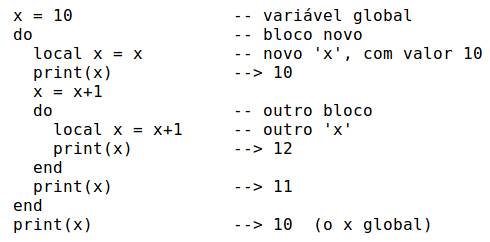
\includegraphics[width=0.5\linewidth]{imagens/imagem3.png}
\caption{Verificação de escopo em Lua}
\end{figure}

Note que, em uma declaração como local x = x, o novo x sendo declarado não está no escopo ainda e portanto o segundo x se refere a uma variável externa.

Por causa das regras de escopo léxico, variáveis locais podem ser livremente acessadas por funções definidas dentro do seu escopo. Uma variável local usada por uma função mais interna é chamada de upvalue ou variável local externa, dentro da função mais interna.

\chapter{Tipos de Dados em Lua}
Os tipos de dados de uma linguagem de programação, são um dos fatores de maior importância para determinar a facilidade com que os programas podem executar problemas do mundo real. Pois para algumas aplicações certos tipos de dados conseguem mapear bem um tipo de problema. Portanto é imprescindível que uma linguagem suporte vários tipos de dados e estruturas.

Existem oito tipos de dados básicos em Lua, são eles, nil, boolean, number, string, function, userdata, thread e table. Nil é o tipo do valor nulo, cuja propriedade principal é ser diferente de qualquer outro valor, ele geralmente representa a ausência de um valor útil. Boolean é o tipo dos valores false e true. Tanto nil como false tornam uma condição falsa, sendo que, qualquer outro valor torna a condição verdadeira. Number representa números reais (ponto flutuante de precisão dupla). O tipo string representa cadeias de caracteres.

O tipo userdata permite que dados C arbitrários possam ser armazenados em variáveis Lua. Este tipo corresponde a um bloco de memória e não tem operações pré-definidas em Lua. O tipo thread representa fluxos de execução independentes e é usado para implementar co-rotinas. Não se pode confundir o tipo thread de Lua com os processos leves do sistema operacional, pois Lua dá suporte a co-rotinas em todos os sistemas.

O tipo table implementa arrays associativos, isto é, arrays que podem ser indexados não apenas por números, mas por qualquer valor (exceto nil). Tabelas podem ser heterogêneas, ou seja, elas podem conter valores de todos os tipos (exceto nil). Tabelas são o único mecanismo de estruturação de dados em Lua, todavia, elas podem ser usadas para representar arrays comuns, tabelas de símbolos, conjuntos, registros, grafos, árvores, etc.

\chapter{Expressões}
Uma expressão em linguagens de programação é uma combinação de valores, variáveis, operadores e chamadas de funções que são interpretadas de acordo com as ordens de precedência e de associatividade particulares a uma determinada linguagem, que calcula e, em seguida, retorna um valor.

As expressões básicas em Lua, já vistas na sintaxe da linguagem são as seguintes:
\begin{itemize}
\item exp ::= expprefixo
\item exp ::= nil | false | true
\item exp ::= Numero
\item exp ::= Cadeia
\item exp ::= funcao
\item exp ::= construtortabela
\item exp ::= ...
\item exp ::= exp opbin exp
\item exp ::= opunaria exp
\item expprefixo ::= var | chamadadefuncao | ( exp )
\end{itemize}

Em virtude do que foi apresentado abordaremos agora algumas operações importantes que encontramos nas expressões.

\section{Operadores Aritméticos}
A linguagem Lua fornece os principais elementos de aritméticos binários como a adição (+), subtração (-), multiplicação (*), divisão (/), módulo (\%) e exponenciação (\^ ), além do aperador unário de negação (-). Se os operandos são números ou cadeias de caracteres que podem ser convertidas para números, então todas as operações possuem o seu significado usual.

\section{Operadores Relacionais}
Um operador relacional compara os valores de dois operandos, sendo que o valor da expressão relacional é booleano. Os operadores relacionais em Lua são:

\begin{itemize}
  \item ==
  \item \~=
  \item <
  \item >
  \item <=
  \item >=
\end{itemize}

Estes operadores sempre possuem como resultado \textbf{true} ou \textbf{false}.

A igualdade (==) primeiro compara o tipo dos operandos envolvidos na comparação. Logo, se os tipos são diferentes, então o resultado é \textbf{false}. Caso contrário, os valores dos operandos são comparados. Números e cadeias de caracteres são comparados de maneira usual. Objetos (valores do tipo table, userdata, thread e function) são comparados por referência, porque dois objetos são considerados iguais somente se eles são o mesmo objeto. Sendo assim, todas as vezes que um novo objeto é criado este novo objeto é diferente de qualquer outro objeto que existia anteriormente.

\section{Operadores Lógicos}
Os operadores lógicos em Lua são \textbf{and}, \textbf{or} e \textbf{not}. Sendo que, todos os operadores lógicos consideram false e nil como falso e qualquer outro valor diferente como verdadeiro.

O operador de negação \textbf{not} sempre retorna false ou true. Já o operador de conjunção \textbf{and} retorna seu primeiro argumento, se este valor é false ou nil, caso contrário o operador retorna o segundo argumento. Todavia, o operador \textbf{or} retorna seu primeiro argumento se o valor deste é diferente de nil e de false, caso contrário, retorna o seu segundo argumento. Tanto and como or usam avaliação de curto-circuito, isto é, o segundo operando é avaliado somente quando é necessário. Aqui estão alguns exemplos:

10 or 20            --> 10

10 or error()       --> 10

nil or ``a''        --> ``a''

nil and 10          --> nil

false and error()   --> false

false and nil       --> false

false or nil        --> nil

10 and 20           --> 20

\section{Concatenação e Operador de Comprimento}
O operador de concatenação de cadeias de caracteres em Lua é denotado por dois pontos (..) . Se ambos os operandos são cadeias de caracteres ou números, então eles são convertidos para cadeias de caracteres.

Com base no que foi mencionado observe o seguinte exemplo:

\begin{figure}[H]
\centering
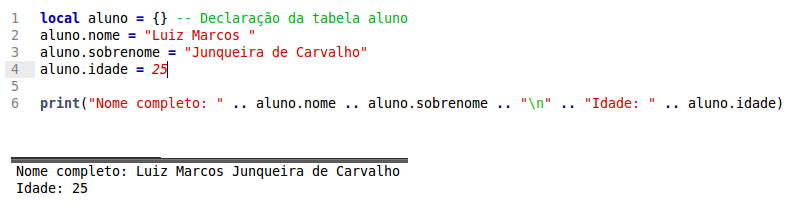
\includegraphics[width=1\linewidth]{imagens/concatenacao.png}
\caption{Concatenação de variáveis com cadeia de caracteres}
\end{figure}

O operador de comprimento é denotado pelo operador unário \#. O comprimento de uma cadeia de caracteres, por exemplo é o seu número de bytes. O comprimento de uma tabela t é definido como qualquer índice inteiro n tal que t[n] não é nil e t[n+1] é nil, além disso, se t[1] é nil, n pode ser zero. Para um array comum, com todos os valores diferentes de nil indo de 1 até n, o seu comprimento é exatamente n. Se o array possuir intervalos descontínuos, então \#t pode ser qualquer um dos índices que imediatamente precedem um valor nil.

\section{Precedência}
A precedência de operadores em Lua segue a \textit{Tabela 1} na página seguinte, na ordem de menor prioridade para a maior:
\begin{table}
\centering
\begin{tabular}{c|c|c|c|c|c}
\hline
\multicolumn{6}{|c|}{\textbf{Tabela de Precedência}} \\
\hline
\multicolumn{6}{|c|}{or} \\
\hline
\multicolumn{6}{|c|}{and} \\
\hline
\multicolumn{6}{|c|}{< \textit{ou} > \textit{ou} <= \textit{ou} >= \textit{ou} \~= \textit{ou} ==} \\
\hline
\multicolumn{6}{|c|}{..} \\
\hline
\multicolumn{6}{|c|}{+ \textit{ou} -} \\
\hline
\multicolumn{6}{|c|}{* \textit{ou} / \textit{ou} \%} \\
\hline
\multicolumn{6}{|c|}{not \textit{ou} \# \textit{ou} -(unary)} \\
\hline
\multicolumn{6}{|c|}{\^.} \\
\end{tabular}
\label{completa}
\caption{Tabela de precedência em Lua}
\end{table}

Como padrão, não existe a necessidade de usar parênteses para mudar as precedências de uma expressão. Os operadores de concatenação e de exponenciação são associativos à direita. Todos os demais operadores binários são associativos à esquerda.

\section{Definições e Chamadas de Função}
A sintaxe para a definição de uma função é

  funcao ::= function corpodafuncao
  funcao ::= ( [listapar] ) bloco end

Podemos verificar em Lua que o comando \textbf{function f () corpo end} é traduzido para \textbf{f = function () corpo end}

Uma definição de função é uma expressão executável, cujo valor tem tipo function. Quando Lua pré-compila um trecho, todos os corpos das funções do trecho são pré-compilados também. Então, sempre que Lua executa a definição de uma função, a função é instanciada (ou fechada).

Uma chamada de função em Lua tem a seguinte sintaxe:

  chamadadefuncao ::= expprefixo args

Em uma chamada de função, primeiro \textbf{expprefixo} e \textbf{args} são avaliados. Se o valor de \textbf{expprefixo} possui tipo function, então esta função é chamada com os argumentos fornecidos, conforme o exemplo abaixo:

\begin{figure}[H]
\centering
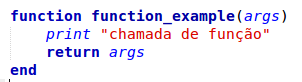
\includegraphics[width=0.5\linewidth]{imagens/function.png}
\caption{Chamada de Função em Lua}
\end{figure}

Uma chamada de funcao da forma return é denominada de chamada final. Portanto, Lua implementa chamadas finais próprias em uma chamada final, logo a função chamada reusa a entrada na pilha da função que a chamou. Sendo assim, não há limite no número de chamadas finais aninhadas que um programa pode executar. Note que uma chamada final somente acontece com uma sintaxe particular, onde o return possui uma única chamada de função como argumento.

\chapter{Sentenças de Atribuição}
\chapter{Estruturas de Controle}
\chapter{Orientação à Tabelas}


\bookmarksetup{startatroot}
% ---

% ---
% Conclusão
% ---
\chapter{Conclusão}


% ----------------------------------------------------------
% ELEMENTOS PÓS-TEXTUAIS
% ----------------------------------------------------------
\postextual


% ----------------------------------------------------------
% Referências bibliográficas
% ----------------------------------------------------------
\bibliography{referencia}


% ----------------------------------------------------------
% Apêndices
% ----------------------------------------------------------

% ---
% Inicia os apêndices
% ---
% \begin{apendicesenv}

% % ----------------------------------------------------------
% \chapter{apendice 1}
% % ----------------------------------------------------------

% paradgmas

% % ----------------------------------------------------------
% \chapter{apendice 2}
% % ----------------------------------------------------------

% paradgmas

% \end{apendicesenv}
% ---


% ----------------------------------------------------------
% Anexos
% ----------------------------------------------------------

% ---
% Inicia os anexos
% ---
\begin{anexosenv}


% \chapter{anexo 1 - Programa Gráfico Mestre}


% \chapter{anexo 2 - Trecho de código da linguagem SOL}


% \chapter{anexo 1}


\end{anexosenv}

%---------------------------------------------------------------------
% INDICE REMISSIVO
%---------------------------------------------------------------------

\printindex

\end{document}

